% GENERATED by data/scripts/eval/gen_scale_all.py -- do not edit.
% Q4 scalability in regex-set size (input fixed), per folding step.
% Two-column figure*: columns = datasets (ClamAV | MS-DLP), rows =
% metrics (top: absolute R1CS with single-rule floor; bottom: net R1CS
% per rule-byte). One curve per corpus (dense / sparse). Lookup share
% excluded (one-time, amortized). All numbers derived from logs.
\begin{figure*}[t]
\centering
\begin{minipage}[t]{\columnwidth}
\centering
{\small \textsc{ClamAV}}\par
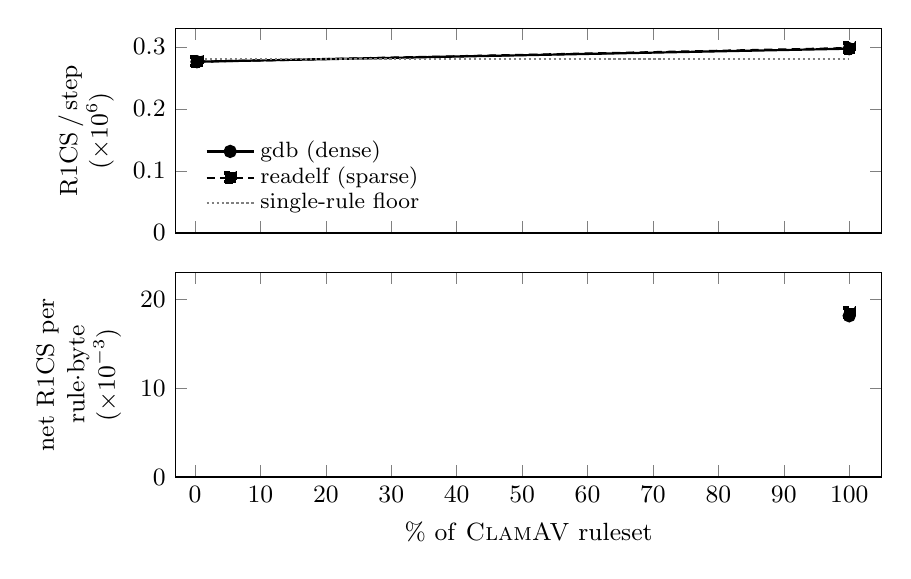
\begin{tikzpicture}[baseline=(ptop.north west)]
% --- top: absolute per-step circuit size ---
\begin{axis}[
    name=ptop, scale only axis, width=0.74\columnwidth, height=2.6cm,
    xmin=-3, xmax=105, xtick={0,10,20,30,40,50,60,70,80,90,100}, xticklabels={},
    ymin=0, ymax=0.33, ylabel={R1CS\,/\,step\\($\times10^{6}$)}, ylabel style={font=\small, align=center}, 
    tick label style={font=\small}, label style={font=\small},
    legend style={font=\footnotesize, at={(0.03,0.04)}, anchor=south west, draw=none, fill=none, row sep=-2pt}, legend cell align=left]
  \addplot[mark=*, thick] coordinates {(0.3,0.276)(100.0,0.297)};
  \addlegendentry{gdb (dense)}
  \addplot[mark=square*, thick, densely dashed] coordinates {(0.3,0.276)(100.0,0.298)};
  \addlegendentry{readelf (sparse)}
  \addplot[gray, densely dotted, thick] coordinates {(0,0.28)(100,0.28)};
  \addlegendentry{single-rule floor}
\end{axis}
% --- bottom: net R1CS per rule-byte (amortization) ---
\begin{axis}[
    name=pbot, scale only axis, width=0.74\columnwidth, height=2.6cm,
    at={(ptop.south west)}, anchor=north west, yshift=-0.5cm,
    xmin=-3, xmax=105, xtick={0,10,20,30,40,50,60,70,80,90,100},
    xlabel={\% of \textsc{ClamAV} ruleset},
    ymin=0, ymax=23.0, ylabel={net R1CS per\\rule$\cdot$byte\\($\times10^{-3}$)}, ylabel style={font=\small, align=center}, 
    tick label style={font=\small}, label style={font=\small}]
  \addplot[mark=*, thick] coordinates {(100.0,18.115)};
  \addplot[mark=square*, thick, densely dashed] coordinates {(100.0,18.423)};
\end{axis}
\end{tikzpicture}
\end{minipage}
\hfill
\begin{minipage}[t]{\columnwidth}
\centering
{\small \textsc{MS-DLP}}\par
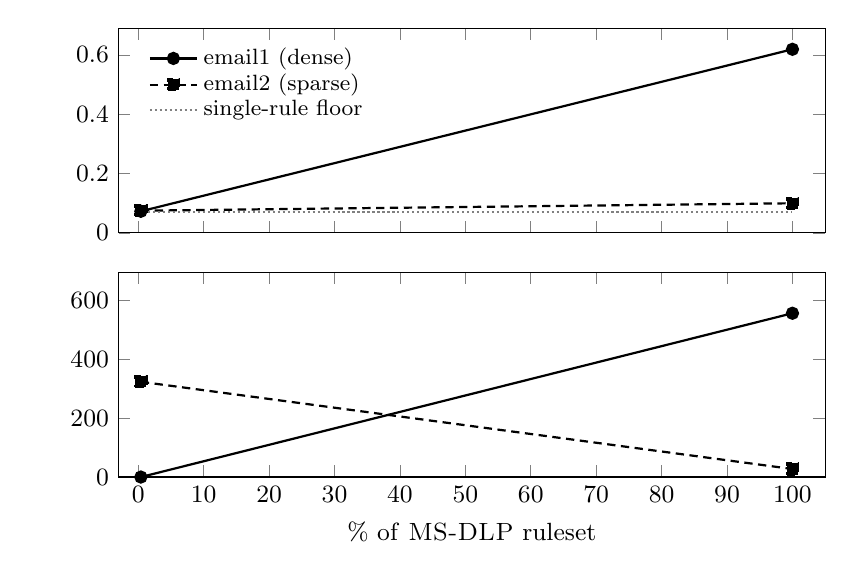
\begin{tikzpicture}[baseline=(ptop.north west)]
% --- top: absolute per-step circuit size ---
\begin{axis}[
    name=ptop, scale only axis, width=0.74\columnwidth, height=2.6cm,
    xmin=-3, xmax=105, xtick={0,10,20,30,40,50,60,70,80,90,100}, xticklabels={},
    ymin=0, ymax=0.69, yticklabel style={text width=2.6em, align=right}, 
    tick label style={font=\small}, label style={font=\small},
    legend style={font=\footnotesize, at={(0.03,0.96)}, anchor=north west, draw=none, fill=none, row sep=-2pt}, legend cell align=left]
  \addplot[mark=*, thick] coordinates {(0.4,0.073)(100.0,0.619)};
  \addlegendentry{email1 (dense)}
  \addplot[mark=square*, thick, densely dashed] coordinates {(0.4,0.075)(100.0,0.100)};
  \addlegendentry{email2 (sparse)}
  \addplot[gray, densely dotted, thick] coordinates {(0,0.07)(100,0.07)};
  \addlegendentry{single-rule floor}
\end{axis}
% --- bottom: net R1CS per rule-byte (amortization) ---
\begin{axis}[
    name=pbot, scale only axis, width=0.74\columnwidth, height=2.6cm,
    at={(ptop.south west)}, anchor=north west, yshift=-0.5cm,
    xmin=-3, xmax=105, xtick={0,10,20,30,40,50,60,70,80,90,100},
    xlabel={\% of \textsc{MS-DLP} ruleset},
    ymin=0, ymax=695.5, yticklabel style={text width=2.6em, align=right}, 
    tick label style={font=\small}, label style={font=\small}]
  \addplot[mark=*, thick] coordinates {(0.4,0.000)(100.0,556.387)};
  \addplot[mark=square*, thick, densely dashed] coordinates {(0.4,323.589)(100.0,27.241)};
\end{axis}
\end{tikzpicture}
\end{minipage}
\caption{Ruleset-size scalability (input fixed), per folding step, on \textsc{ClamAV} (left) and \textsc{MS-DLP} (right). \emph{Top:} absolute circuit size with the single-rule framework floor (dotted; $0.28$\,M R1CS for \textsc{ClamAV}, $0.07$\,M for \textsc{MS-DLP}); growing the ruleset to the full $300$ (\textsc{ClamAV}) / $494$ (\textsc{MS-DLP}) rules grows the circuit far slower than the rule count. \emph{Bottom:} net circuit cost \emph{per rule per input byte}---cumulative R1CS above the floor divided by cumulative rule count times per-step input length---falling from $18.11\times10^{-3}$ to $18.11\times10^{-3}$ (\ttt{gdb}) and $18.42\times10^{-3}$ to $18.42\times10^{-3}$ (\ttt{readelf}) R1CS per rule-byte (\textsc{ClamAV}) and $556.39\times10^{-3}$ to $556.39\times10^{-3}$ (\ttt{email1}) and $323.59\times10^{-3}$ to $27.24\times10^{-3}$ (\ttt{email2}) R1CS per rule-byte (\textsc{MS-DLP}) at the full set. For the same \textsc{MS-DLP} ruleset, \textsc{Zombie} emits $3{,}407{,}872$ R1CS in total; dividing by the $2000$-byte input and the same $494$ rules gives $\sim$$3.45$ R1CS per rule-byte, the same normalization applied to BORA.}
\label{fig:scale-regex}
\end{figure*}
